\section{Yêu cầu khai thác}
%%%%%%%%%%%%%%%%%%%%%%%%%%%%%%%%%%%%%%%%%%%%%%%%%%%%%%
    \subsection{Động lực, mục tiêu chính và phạm vi dự án}
%%%%%%%%%%%%%%%%%%%%%%%%%%%%%%%%%%%%%%%%%%%%%%%%%%%%%%
% Động lực dự án
%%%%%%%%%%%%%%%%%%%%%%%%%%%%%%%%%%%%%%%%%%%%%%%%%%%%%%
        \subsubsection{Động lực dự án}
            Trong bối cảnh xu hướng thế giới là mua sắm trực tuyến, các doanh nghiệp đang chú trọng hơn trong nền tảng này. Do đó việc có một nền tảng thương mại điện tử thân thiện và hiệu quả với người dùng là điều cực kỳ cần thiết để các doanh nghiệp có thể tiếp cận khách hàng một cách dễ dàng hơn và cũng như là để khách hàng mua được các sản phẩm của các nhãn hàng một cách nhanh chóng. Và trong tất cả các mặt hàng thì áo quần là mặt hàng có nhu cầu cao nhất. Dự án này ra đời với mục tiêu giúp các doanh nghiệp may mặc tận dụng được lợi thế của công nghệ để tăng trưởng doanh số, tối ưu hóa quy trình bán hàng, mở rộng thị trường và giúp cho thương hiệu được nhiều người biết tới.\\
        \subsubsection{Mục tiêu chính của dự án}
            Dự án này tập trung phát triển một nền tảng thương mại điện tử, hỗ trợ các chức năng như quản lý sản phẩm, đơn hàng, tích hợp các phương thức thanh toán, thông báo tự động. Dự án cũng cung cấp giao diện mua sắm thân thiện cho người dùng, tích hợp nhiều phương thức thanh toán đồng thời cung cấp các chức năng quản lý hệ thống cho nhà quản trị nền tảng.\\
        \subsubsection{Phạm vi dự án}
            Dự án phát triển sử dụng công nghệ PERN Stack nhằm phát triển một nền tảng sàn thương mại điện tử cho nhiều nhãn hàng áo quần. Nền tảng sẽ cho phép khách hàng tìm kiếm, mua sắm và thực hiện các giao dịch thanh toán trực tuyến một cách tiện lợi. Đồng thời dự án cũng chú trọng việc tối ưu hóa quy trình quản lý cho nhà quản trị sàn thương mại.\\
            \begin{enumerate}[label=\arabic{section}.\arabic{subsection}.\arabic{subsubsection}.\alph*, leftmargin=3cm]
                \item \textbf{Tính năng chính} \\
                    - Phát triển hệ thống quản lý sản phẩm, đơn hàng: Hệ thống sẽ bao gồm các tính năng cho phép chủ cửa hàng thêm mới, chỉnh sửa và xóa các sản phẩm, đơn hàng đồng thời chủ cửa hàng có thể quản lý kho hàng một cách dễ dàng. Điều này cho phép các cửa hàng theo dõi được tình trạng hàng hóa trong kho một cách chính xác, tự động cập nhật số lượng sau mỗi đơn hàng. \\
                    - Xây dựng tính năng xử lí đơn hàng: Từ khi người mua đặt hàng, hệ thống sẽ ghi nhận đơn hàng và xử lí thanh toán rồi theo dõi trạng thái đơn hàng (đang xử lý, đang giao, đã giao, hủy/đổi hàng,...). Các thông tin về đơn hàng cũng được cập nhật cho khách hàng để họ có thể theo dõi tiến độ. \\
                    - Tích hợp phương thức thanh toán trực tuyến: Hệ thống sẽ hỗ trợ phương thức thanh toán trực tuyến. Điều này giúp người dùng linh hoạt hơn trong việc thanh toán đồng thời tăng tính tiện lợi của nền tảng. \\
                    - Tìm kiếm: Hỗ trợ công cụ tìm kiếm nhanh gọn, cho phép người dùng nhập tên sản phẩm hoặc từ khóa liên quan để hiện thị kết quả. Công cụ tìm kiếm tập trung vào tốc độ và sự chính xác giúp người dùng tìm thấy sản phẩm mà không cần qua nhiều bước phức tạp. \\
                    - Giao diện người dùng trực quan và tối ưu hóa trải nghiệm: Giao diện sẽ được thiết kế đơn giản, dễ sử dụng, giúp người dùng tìm kiếm và mua bán nhanh chóng. \\
                    - Quản lý hệ thống: Hệ thống cung cấp các chức năng quản lý người dùng và hệ thống trực quan, dễ sử dụng giúp cho các quản trị viên có thể làm quen với công cụ. Đồng thời giúp quản trị viên dễ dàng xử lí các báo cáo, khiếu nại.
                    - Đảm bảo bảo mật và bảo vệ dữ liệu quan trọng: Hệ thống tuân thủ các tiêu chuẩn an ninh dữ liệu, đảm bảo thông tin cá nhân và tài chính của người dùng được mã hóa và bảo mật, khó đánh cắp. \\
                \item \textbf{Tích hợp hệ thống} \\
                    - Tích hợp thanh toán: Tích hợp với cổng thanh toán để hỗ trợ các giao dịch thanh toán. Người dùng có thể thực hiện thanh toán trực tuyến. \\
                \item \textbf{Phạm vi người dùng (User Scope)} \\
                    - Khách hàng: Khách hàng có thể tìm kiếm và mua sắm sản phẩm trực tuyến, thanh toán, theo dõi đơn hàng, đánh giá bình luận đơn hàng. \\
                    - Chủ cửa hàng: Cửa hàng có thể quản lý sản phẩm, đơn hàng, kho hàng.
                    - Quản trị viên: Các nhà quản trị sẽ có công cụ để quản lý khách hàng, cửa hàng, nội dung trên nền tảng. \\
                \item \textbf{Giới hạn phạm vi} \\
                    Nền tảng yêu cầu phát triển trên các trình duyệt phổ biến như Google Chrome, Cốc Cốc, Firefox, Microsoft Edge,... Đồng thời yêu cầu tối ưu hóa trên các trình duyệt này nhằm đảm bảo trải nghiệm đồng nhất trên các thiết bị khác nhau.\\
            \end{enumerate}
    \subsection{Phân tích hệ thống liên quan \& Mô tả hệ thống \& Use-case hệ thống}
    
            \subsubsection{Phân tích các hệ thống liên quan}
            
            \textbf{Cool Mate} (\href{https://www.coolmate.me/}{https://www.coolmate.me/}) \\
            
                    \begin{figure}[H]
                        \centering    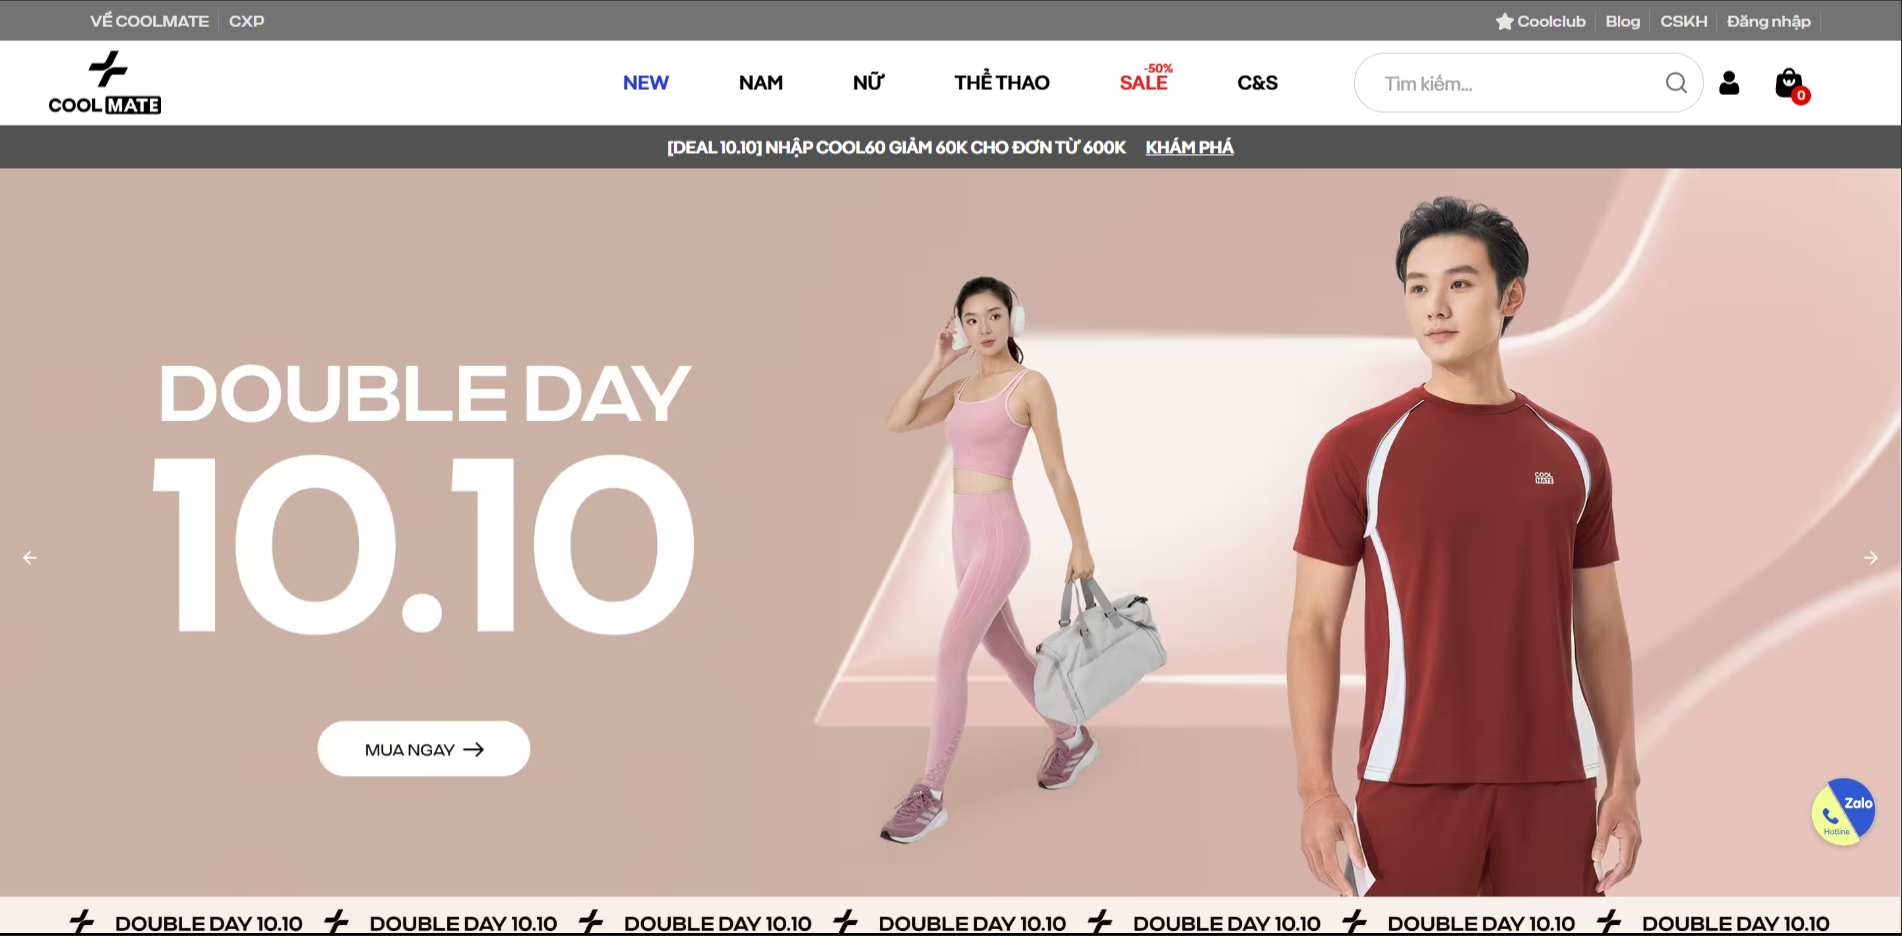
\includegraphics[width=\linewidth]{image/coolmate.png}
                        \label{fig:enter-label}
                        \caption{Trang web CoolMate}
                    \end{figure}
                    
            \begin{adjustwidth}{1.5cm}{0cm} % Lùi toàn bộ phần này vào 1.5cm
            \noindent \textbf{- Ưu điểm}
            \begin{itemize}
                \item Giao diện bắt mắt, trực quan, thân thiện với người dùng.
                \item Hệ thống tìm kiếm hiệu quả.
                \item Tốc độ phản hồi, tải trang nhanh.
            \end{itemize}
            
            \noindent \textbf{- Nhược điểm}
            \begin{itemize}
                \item Nền tảng chỉ của một nhãn hiệu riêng, chưa có sản phẩm đa dạng từ các nhãn hàng khác.
            \end{itemize}
            \end{adjustwidth}

            \textbf{Degrey} (\href{https://degrey.vn/}{https://degrey.vn/}) \\
            
                    \begin{figure}[H]
                        \centering    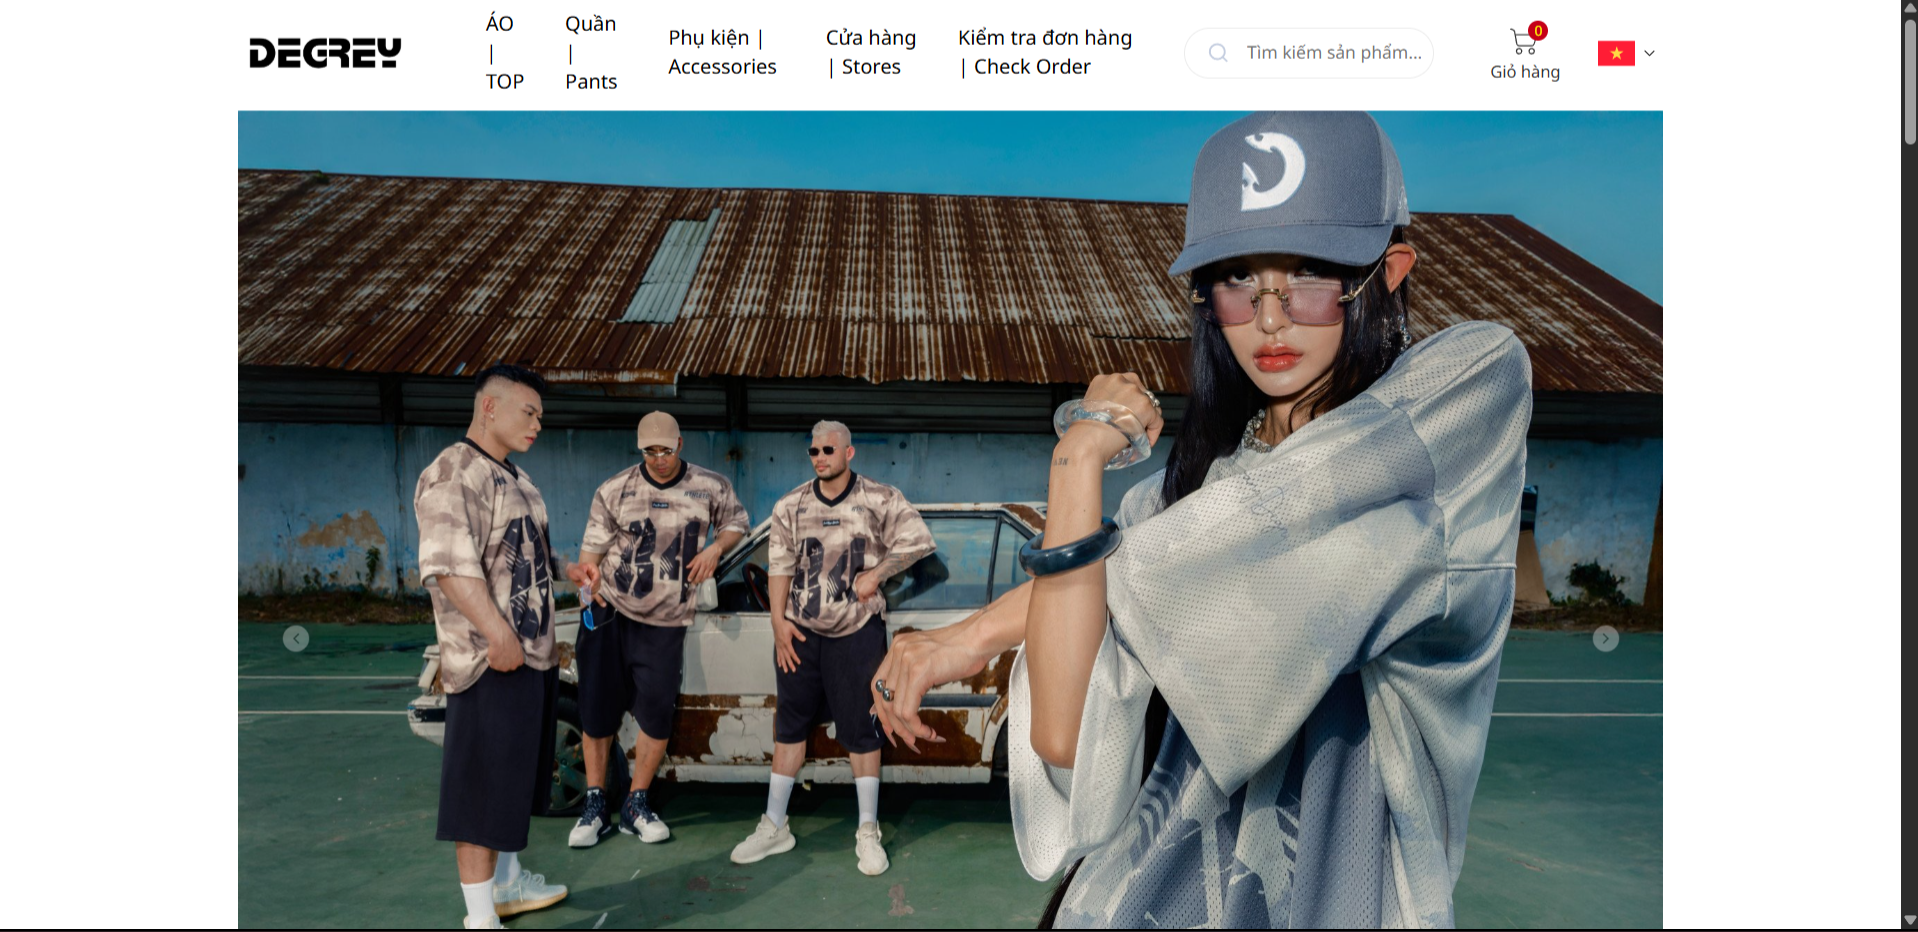
\includegraphics[width=\linewidth]{image/degrey.png}
                        \label{fig:enter-label}
                        \caption{Trang web Degrey}
                    \end{figure}
                    
            \begin{adjustwidth}{1.5cm}{0cm} % Lùi toàn bộ phần này vào 1.5cm
            \noindent \textbf{- Ưu điểm}
            \begin{itemize}
                \item Giao diện bắt mắt, mới lạ, thu hút người mua.
                \item Hệ thống tìm kiếm nhanh chóng, được chưa thành nhiều mục, loại hợp lý.
            \end{itemize}
            
            \noindent \textbf{- Nhược điểm}
            \begin{itemize}
                \item Chưa có hệ thống chat, trao đổi giữa khách hàng và cửa hàng trực tuyến.
            \end{itemize}
            \end{adjustwidth}

            \begin{adjustwidth}{1.5cm}{0cm}
                \textbf{Các kinh nghiệm áp dụng vào hệ thống: } Hệ thống của nhóm sẽ học hỏi các điểm mạnh, tốt của hai trang web trên đồng thời cải thiện điểm yếu của các trang web trên. Ví dụ như là cho phép nhiều nhãn hàng hoạt động trên nền tảng để tăng độ đa dạng sản phẩm và tích hợp hệ thống trao đổi, chat giữa khách hàng và các cửa hàng. \\
            \end{adjustwidth}
            
            \subsubsection{Các yêu cầu chức năng \& phi chức năng}
                \hspace{1.5cm} Các đổi tượng sử dụng: Khách hàng, Cửa hàng, Admin.
                \begin{enumerate}[label=\arabic{section}.\arabic{subsection}.\arabic{subsubsection}.\alph*,leftmargin=3cm]
                    \item \textbf{Yêu cầu chức năng} \\
                        \textbf{Chức năng chung:}
                        \begin{itemize}
                            \item Đăng ký, đăng nhập, đăng xuất $\rightarrow$ 
                            Authentication
                            \item Phân quyền
                            \item Tìm kiếm sản phẩm
                        \end{itemize}
    
                        \textbf{Khách hàng:}
                        \begin{itemize}
                            \item Nhận thông báo về đơn hàng từ hệ thống
                            \item Thêm vào  giỏ hàng
                            \item Đặt hàng, thanh toán( Lựa chọn nhiều phương thức tích hợp sẵn hoặc là ship cod)
                            \item Bình luận, đánh giá sản phẩm
                            \item Yêu cầu hỗ trợ (Hủy đổi, trả hàng,...)
                        \end{itemize}

                        \textbf{Cửa hàng:}
                        \begin{itemize}
                            \item Thiết lập thông tin của cửa hàng
                            \item Quản lý sản phẩm(thông tin cơ bản, số lượng,...)
                            \item Quản lý đơn hàng(xác nhận, hủy đơn hàng, theo dõi trạng thái đơn hàng,...)
                        \end{itemize}

                        \textbf{Admin:}
                        \begin{itemize}
                            \item Quản lý tài khoản, thông tin khách hàng
                            \item Quản lý các cửa hàng
                            \item Quản lý các nội dung, sản phẩm trên nền tảng
                            \item Xử lí các báo cáo của khách hàng
                        \end{itemize}
                    \item \textbf{Yêu cầu phi chức năng} \\
                    \textbf{Bảo mật}\\
                        - Dữ liệu người dùng đặc biệt mật khẩu cần được mã hóa trước khi lưu vào cơ sở dữ liệu \\
                        - Giới hạn thời gian của một phiên đăng nhập là 2h, hết hạn thì cần đăng nhập lại. \\
                    \textbf{Hiệu suất}\\
                        - Hệ thống phải đáp ứng tối thiểu 500 người dùng đồng thời \\
                        - Thời gian phản hồi trung bình cho mỗi request không quá 3 giây. \\
                        - Với kết nối thông thường thì phải tải xong trang chủ trong vòng 2 giây. \\
                    \textbf{Khả năng tương thích}\\
                        - Trang web hoạt động tốt với phiên bản mới nhất của các trình duyệt phổ biến như Google Chrome, Cốc Cốc, Firefox,... \\
                    \textbf{Khả năng sử dụng}\\
                        - Trang web phải dễ sử dụng và làm quen cho người dùng, chỉ cần khoảng 10-20 phút để thành thạo các thao tác cơ bản.\\
                        - Các nút bấm cần được làm nổi bật để người dùng dễ thấy \\
                        - Các thao tác cần đơn giản không rườm rà, giảm bớt các thao tác thừa không cần có \\
                \end{enumerate}
            \subsubsection{Use-case hệ thống}
                \begin{figure}[H]
                \centering    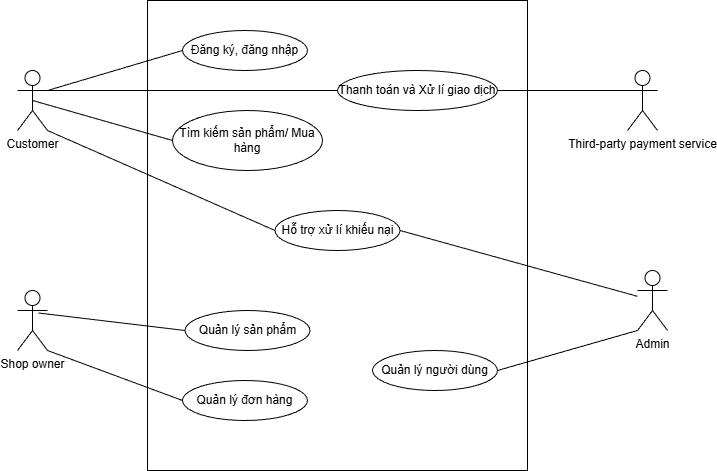
\includegraphics[width=\linewidth]{image/USE_CASE_SYSTEM.drawio.png}
                \label{fig:enter-label}
                \caption{Diagram use case hệ thống}
                \end{figure}
    \subsection{Use-case diagram \& scenario cho các tính năng chính của hệ thống}
        \subsubsection{Tính năng tìm kiếm và thêm sản phẩm vào giỏ hàng }
    \begin{figure}[H]
    \centering    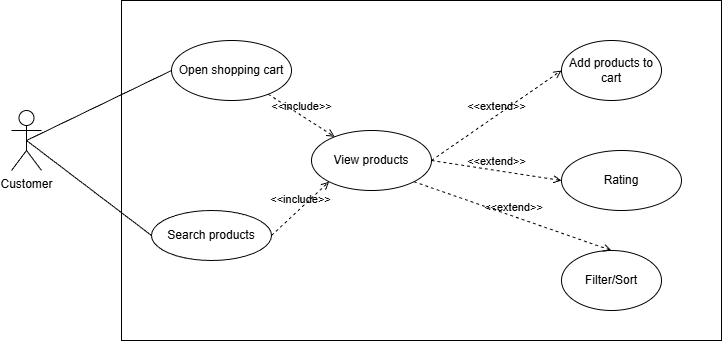
\includegraphics[width=\linewidth]{image/USE_CASE_ADD_PRODUCT.drawio.png}
    \label{fig:enter-label}
    \caption{Diagram use case của tính năng tìm kiếm và thêm sản phẩm vào giỏ hàng}
    \end{figure}
    \begin{longtable}{|>{\bfseries}p{4.5cm}|p{11cm}|} \hline 
Use case name: & Tìm kiếm và thêm sản phẩm vào giỏ hàng \\ \hline
Date created: & 11/10/2025 \\ \hline
Last updated date: & 30/11/2025 \\ \hline
Actor: & Customer \\ \hline
Description: & 
Customer có thể thực hiện mua hàng / thêm sản phẩm vào giỏ hàng / tìm kiếm sản phẩm  \\ \hline
Trigger: & 
Khi customer nhấn chọn biểu tượng " Tìm kiếm" hoặc khi customer chọn biểu tượng sản phẩm  \\ \hline
Pre-conditions: & 

Khách hàng đã đăng nhập vào hệ thống (hoặc có quyền truy cập như khách vãng lai nếu được phép). \newline
Hệ thống hoạt động bình thường, cho phép truy cập danh mục và thông tin sản phẩm. \newline
Dữ liệu về sản phẩm (tên, giá, mô tả, hình ảnh, tồn kho, v.v.) đã tồn tại trong cơ sở dữ liệu.\newline
Đối với các thao tác như thêm vào giỏ hàng (Add to shopping cart) hoặc chọn phương thức thanh toán (Choose payment method), khách hàng cần có giỏ hàng hợp lệ hoặc sản phẩm được chọn trước đó.\newline
Sản phẩm tồn tại. \\ \hline
Post-conditions: & 
Nếu quá trình thao tác thành công: \newline
Hệ thống hiển thị thông tin sản phẩm tương ứng (View product).\newline
Khách hàng có thể lọc sản phẩm (Filter) theo tiêu chí mong muốn.\newline
Khách hàng có thể thêm sản phẩm vào giỏ hàng (Add to shopping cart).\newline
Giỏ hàng được cập nhật và sẵn sàng cho quá trình thanh toán.\newline
Khách hàng có thể đánh giá sản phẩm (Rating) sau khi xem hoặc mua.
\\ \hline
Normal flow: &
1.Customer chọn biểu tượng tìm kiếm trên thanh tìm kiếm\newline
2.Hệ thống hiển thị sản phẩm gợi ý \newline
3. Customer có thể thêm sản phẩm vào giỏ hàng , xem thông tin sản phẩm và thao tác với sản phẩm hoặc giỏ hàng\newline
4.Sau khi trải nghiệm sản phẩm, customer có thể thực hiện đánh giá sản phẩm sau khi nhận hàng
\\ \hline
Alternative flow: &
2a.Nếu không tìm thấy được kết quả phù hợp trong bước tìm kiếm, hệ thống sẽ thông báo "Không tìm thấy sản phẩm", \newline
2b.Thay vì tìm kiếm cơ bản, customer có thể sử dụng filter để lọc sản phẩm\newline
2c.Customer mua trực tiếp không qua giỏ hàng
\\ \hline
Exception: &
Lỗi không tồn tại sản phẩm\newline
Lọc không trả về kết quả\newline
Tài khoản bị khóa nên không thực hiện được tác vụ\newline
Đánh giá không hợp lệ\newline
 \\ \hline
\caption{Đặc tả use case tính năng tìm kiếm/thêm sản phẩm vào giỏ hàng của người dùng }
\end{longtable}

